%%*************************************************************************
%% Legal Notice:
%% This code is offered as-is without any warranty either expressed or
%% implied; without even the implied warranty of MERCHANTABILITY or
%% FITNESS FOR A PARTICULAR PURPOSE! 
%% User assumes all risk.
%% In no event shall IEEE or any contributor to this code be liable for
%% any damages or losses, including, but not limited to, incidental,
%% consequential, or any other damages, resulting from the use or misuse
%% of any information contained here.
%%
%% All comments are the opinions of their respective authors and are not
%% necessarily endorsed by the IEEE.
%%
%% This work is distributed under the LaTeX Project Public License (LPPL)
%% ( http://www.latex-project.org/ ) version 1.3, and may be freely used,
%% distributed and modified. A copy of the LPPL, version 1.3, is included
%% in the base LaTeX documentation of all distributions of LaTeX released
%% 2003/12/01 or later.
%% Retain all contribution notices and credits.
%% ** Modified files should be clearly indicated as such, including  **
%% ** renaming them and changing author support contact information. **
%%
%% File list of work: IEEEtran.cls, IEEEtran_HOWTO.pdf, bare_adv.tex,
%%                    bare_conf.tex, bare_jrnl.tex, bare_jrnl_compsoc.tex,
%%                    bare_jrnl_transmag.tex
%%*************************************************************************

% Note that the a4paper option is mainly intended so that authors in
% countries using A4 can easily print to A4 and see how their papers will
% look in print - the typesetting of the document will not typically be
% affected with changes in paper size (but the bottom and side margins will).
% Use the testflow package mentioned above to verify correct handling of
% both paper sizes by the user's LaTeX system.
%
% Also note that the "draftcls" or "draftclsnofoot", not "draft", option
% should be used if it is desired that the figures are to be displayed in
% draft mode.
%
\documentclass[journal]{IEEEtran}
%
% If IEEEtran.cls has not been installed into the LaTeX system files,
% manually specify the path to it like:
% \documentclass[journal]{../sty/IEEEtran}





% Some very useful LaTeX packages include:
% (uncomment the ones you want to load)


% *** MISC UTILITY PACKAGES ***
%
%\usepackage{ifpdf}
% Heiko Oberdiek's ifpdf.sty is very useful if you need conditional
% compilation based on whether the output is pdf or dvi.
% usage:
% \ifpdf
%   % pdf code
% \else
%   % dvi code
% \fi
% The latest version of ifpdf.sty can be obtained from:
% http://www.ctan.org/tex-archive/macros/latex/contrib/oberdiek/
% Also, note that IEEEtran.cls V1.7 and later provides a builtin
% \ifCLASSINFOpdf conditional that works the same way.
% When switching from latex to pdflatex and vice-versa, the compiler may
% have to be run twice to clear warning/error messages.






% *** CITATION PACKAGES ***
%
%\usepackage{cite}
% cite.sty was written by Donald Arseneau
% V1.6 and later of IEEEtran pre-defines the format of the cite.sty package
% \cite{} output to follow that of IEEE. Loading the cite package will
% result in citation numbers being automatically sorted and properly
% "compressed/ranged". e.g., [1], [9], [2], [7], [5], [6] without using
% cite.sty will become [1], [2], [5]--[7], [9] using cite.sty. cite.sty's
% \cite will automatically add leading space, if needed. Use cite.sty's
% noadjust option (cite.sty V3.8 and later) if you want to turn this off
% such as if a citation ever needs to be enclosed in parenthesis.
% cite.sty is already installed on most LaTeX systems. Be sure and use
% version 4.0 (2003-05-27) and later if using hyperref.sty. cite.sty does
% not currently provide for hyperlinked citations.
% The latest version can be obtained at:
% http://www.ctan.org/tex-archive/macros/latex/contrib/cite/
% The documentation is contained in the cite.sty file itself.






% *** GRAPHICS RELATED PACKAGES ***
%
\ifCLASSINFOpdf
  % \usepackage[pdftex]{graphicx}
  % declare the path(s) where your graphic files are
  % \graphicspath{{../pdf/}{../jpeg/}}
  % and their extensions so you won't have to specify these with
  % every instance of \includegraphics
  % \DeclareGraphicsExtensions{.pdf,.jpeg,.png}
\else
  % or other class option (dvipsone, dvipdf, if not using dvips). graphicx
  % will default to the driver specified in the system graphics.cfg if no
  % driver is specified.
  % \usepackage[dvips]{graphicx}
  % declare the path(s) where your graphic files are
  % \graphicspath{{../eps/}}
  % and their extensions so you won't have to specify these with
  % every instance of \includegraphics
  % \DeclareGraphicsExtensions{.eps}
\fi
% graphicx was written by David Carlisle and Sebastian Rahtz. It is
% required if you want graphics, photos, etc. graphicx.sty is already
% installed on most LaTeX systems. The latest version and documentation
% can be obtained at: 
% http://www.ctan.org/tex-archive/macros/latex/required/graphics/
% Another good source of documentation is "Using Imported Graphics in
% LaTeX2e" by Keith Reckdahl which can be found at:
% http://www.ctan.org/tex-archive/info/epslatex/
%
% latex, and pdflatex in dvi mode, support graphics in encapsulated
% postscript (.eps) format. pdflatex in pdf mode supports graphics
% in .pdf, .jpeg, .png and .mps (metapost) formats. Users should ensure
% that all non-photo figures use a vector format (.eps, .pdf, .mps) and
% not a bitmapped formats (.jpeg, .png). IEEE frowns on bitmapped formats
% which can result in "jaggedy"/blurry rendering of lines and letters as
% well as large increases in file sizes.
%
% You can find documentation about the pdfTeX application at:
% http://www.tug.org/applications/pdftex





% *** MATH PACKAGES ***
%
%\usepackage[cmex10]{amsmath}
% A popular package from the American Mathematical Society that provides
% many useful and powerful commands for dealing with mathematics. If using
% it, be sure to load this package with the cmex10 option to ensure that
% only type 1 fonts will utilized at all point sizes. Without this option,
% it is possible that some math symbols, particularly those within
% footnotes, will be rendered in bitmap form which will result in a
% document that can not be IEEE Xplore compliant!
%
% Also, note that the amsmath package sets \interdisplaylinepenalty to 10000
% thus preventing page breaks from occurring within multiline equations. Use:
%\interdisplaylinepenalty=2500
% after loading amsmath to restore such page breaks as IEEEtran.cls normally
% does. amsmath.sty is already installed on most LaTeX systems. The latest
% version and documentation can be obtained at:
% http://www.ctan.org/tex-archive/macros/latex/required/amslatex/math/





% *** SPECIALIZED LIST PACKAGES ***
%
%\usepackage{algorithmic}
% algorithmic.sty was written by Peter Williams and Rogerio Brito.
% This package provides an algorithmic environment fo describing algorithms.
% You can use the algorithmic environment in-text or within a figure
% environment to provide for a floating algorithm. Do NOT use the algorithm
% floating environment provided by algorithm.sty (by the same authors) or
% algorithm2e.sty (by Christophe Fiorio) as IEEE does not use dedicated
% algorithm float types and packages that provide these will not provide
% correct IEEE style captions. The latest version and documentation of
% algorithmic.sty can be obtained at:
% http://www.ctan.org/tex-archive/macros/latex/contrib/algorithms/
% There is also a support site at:
% http://algorithms.berlios.de/index.html
% Also of interest may be the (relatively newer and more customizable)
% algorithmicx.sty package by Szasz Janos:
% http://www.ctan.org/tex-archive/macros/latex/contrib/algorithmicx/




% *** ALIGNMENT PACKAGES ***
%
%\usepackage{array}
% Frank Mittelbach's and David Carlisle's array.sty patches and improves
% the standard LaTeX2e array and tabular environments to provide better
% appearance and additional user controls. As the default LaTeX2e table
% generation code is lacking to the point of almost being broken with
% respect to the quality of the end results, all users are strongly
% advised to use an enhanced (at the very least that provided by array.sty)
% set of table tools. array.sty is already installed on most systems. The
% latest version and documentation can be obtained at:
% http://www.ctan.org/tex-archive/macros/latex/required/tools/


% IEEEtran contains the IEEEeqnarray family of commands that can be used to
% generate multiline equations as well as matrices, tables, etc., of high
% quality.




% *** SUBFIGURE PACKAGES ***
%\ifCLASSOPTIONcompsoc
%  \usepackage[caption=false,font=normalsize,labelfont=sf,textfont=sf]{subfig}
%\else
%  \usepackage[caption=false,font=footnotesize]{subfig}
%\fi
% subfig.sty, written by Steven Douglas Cochran, is the modern replacement
% for subfigure.sty, the latter of which is no longer maintained and is
% incompatible with some LaTeX packages including fixltx2e. However,
% subfig.sty requires and automatically loads Axel Sommerfeldt's caption.sty
% which will override IEEEtran.cls' handling of captions and this will result
% in non-IEEE style figure/table captions. To prevent this problem, be sure
% and invoke subfig.sty's "caption=false" package option (available since
% subfig.sty version 1.3, 2005/06/28) as this is will preserve IEEEtran.cls
% handling of captions.
% Note that the Computer Society format requires a larger sans serif font
% than the serif footnote size font used in traditional IEEE formatting
% and thus the need to invoke different subfig.sty package options depending
% on whether compsoc mode has been enabled.
%
% The latest version and documentation of subfig.sty can be obtained at:
% http://www.ctan.org/tex-archive/macros/latex/contrib/subfig/




% *** FLOAT PACKAGES ***
%
%\usepackage{fixltx2e}
% fixltx2e, the successor to the earlier fix2col.sty, was written by
% Frank Mittelbach and David Carlisle. This package corrects a few problems
% in the LaTeX2e kernel, the most notable of which is that in current
% LaTeX2e releases, the ordering of single and double column floats is not
% guaranteed to be preserved. Thus, an unpatched LaTeX2e can allow a
% single column figure to be placed prior to an earlier double column
% figure. The latest version and documentation can be found at:
% http://www.ctan.org/tex-archive/macros/latex/base/


%\usepackage{stfloats}
% stfloats.sty was written by Sigitas Tolusis. This package gives LaTeX2e
% the ability to do double column floats at the bottom of the page as well
% as the top. (e.g., "\begin{figure*}[!b]" is not normally possible in
% LaTeX2e). It also provides a command:
%\fnbelowfloat
% to enable the placement of footnotes below bottom floats (the standard
% LaTeX2e kernel puts them above bottom floats). This is an invasive package
% which rewrites many portions of the LaTeX2e float routines. It may not work
% with other packages that modify the LaTeX2e float routines. The latest
% version and documentation can be obtained at:
% http://www.ctan.org/tex-archive/macros/latex/contrib/sttools/
% Do not use the stfloats baselinefloat ability as IEEE does not allow
% \baselineskip to stretch. Authors submitting work to the IEEE should note
% that IEEE rarely uses double column equations and that authors should try
% to avoid such use. Do not be tempted to use the cuted.sty or midfloat.sty
% packages (also by Sigitas Tolusis) as IEEE does not format its papers in
% such ways.
% Do not attempt to use stfloats with fixltx2e as they are incompatible.
% Instead, use Morten Hogholm'a dblfloatfix which combines the features
% of both fixltx2e and stfloats:
%
% \usepackage{dblfloatfix}
% The latest version can be found at:
% http://www.ctan.org/tex-archive/macros/latex/contrib/dblfloatfix/




%\ifCLASSOPTIONcaptionsoff
%  \usepackage[nomarkers]{endfloat}
% \let\MYoriglatexcaption\caption
% \renewcommand{\caption}[2][\relax]{\MYoriglatexcaption[#2]{#2}}
%\fi
% endfloat.sty was written by James Darrell McCauley, Jeff Goldberg and 
% Axel Sommerfeldt. This package may be useful when used in conjunction with 
% IEEEtran.cls'  captionsoff option. Some IEEE journals/societies require that
% submissions have lists of figures/tables at the end of the paper and that
% figures/tables without any captions are placed on a page by themselves at
% the end of the document. If needed, the draftcls IEEEtran class option or
% \CLASSINPUTbaselinestretch interface can be used to increase the line
% spacing as well. Be sure and use the nomarkers option of endfloat to
% prevent endfloat from "marking" where the figures would have been placed
% in the text. The two hack lines of code above are a slight modification of
% that suggested by in the endfloat docs (section 8.4.1) to ensure that
% the full captions always appear in the list of figures/tables - even if
% the user used the short optional argument of \caption[]{}.
% IEEE papers do not typically make use of \caption[]'s optional argument,
% so this should not be an issue. A similar trick can be used to disable
% captions of packages such as subfig.sty that lack options to turn off
% the subcaptions:
% For subfig.sty:
% \let\MYorigsubfloat\subfloat
% \renewcommand{\subfloat}[2][\relax]{\MYorigsubfloat[]{#2}}
% However, the above trick will not work if both optional arguments of
% the \subfloat command are used. Furthermore, there needs to be a
% description of each subfigure *somewhere* and endfloat does not add
% subfigure captions to its list of figures. Thus, the best approach is to
% avoid the use of subfigure captions (many IEEE journals avoid them anyway)
% and instead reference/explain all the subfigures within the main caption.
% The latest version of endfloat.sty and its documentation can obtained at:
% http://www.ctan.org/tex-archive/macros/latex/contrib/endfloat/
%
% The IEEEtran \ifCLASSOPTIONcaptionsoff conditional can also be used
% later in the document, say, to conditionally put the References on a 
% page by themselves.




% *** PDF, URL AND HYPERLINK PACKAGES ***
%
%\usepackage{url}
% url.sty was written by Donald Arseneau. It provides better support for
% handling and breaking URLs. url.sty is already installed on most LaTeX
% systems. The latest version and documentation can be obtained at:
% http://www.ctan.org/tex-archive/macros/latex/contrib/url/
% Basically, \url{my_url_here}.




% *** Do not adjust lengths that control margins, column widths, etc. ***
% *** Do not use packages that alter fonts (such as pslatex).         ***
% There should be no need to do such things with IEEEtran.cls V1.6 and later.
% (Unless specifically asked to do so by the journal or conference you plan
% to submit to, of course. )


% correct bad hyphenation here
\hyphenation{optical net-works semiconductor}

\usepackage[utf8]{inputenc}
\usepackage{url}
\usepackage{amsmath}
\usepackage{breqn}
\usepackage{multirow}
\usepackage{graphicx}
\usepackage[justification=centering]{caption}

\begin{document}

%
% paper title
% can use linebreaks \\ within to get better formatting as desired
% Do not put math or special symbols in the title.
\title{Geolocalización de Nodos Inalámbricos}
%
%
% author names and IEEE memberships
% note positions of commas and nonbreaking spaces ( ~ ) LaTeX will not break
% a structure at a ~ so this keeps an author's name from being broken across
% two lines.
% use \thanks{} to gain access to the first footnote area
% a separate \thanks must be used for each paragraph as LaTeX2e's \thanks
% was not built to handle multiple paragraphs
%

\author{Matías Parodi, Guillermo Reisch}

% note the % following the last \IEEEmembership and also \thanks - 
% these prevent an unwanted space from occurring between the last author name
% and the end of the author line. i.e., if you had this:
% 
% \author{....lastname \thanks{...} \thanks{...} }
%                     ^------------^------------^----Do not want these spaces!
%
% a space would be appended to the last name and could cause every name on that
% line to be shifted left slightly. This is one of those "LaTeX things". For
% instance, "\textbf{A} \textbf{B}" will typeset as "A B" not "AB". To get
% "AB" then you have to do: "\textbf{A}\textbf{B}"
% \thanks is no different in this regard, so shield the last } of each \thanks
% that ends a line with a % and do not let a space in before the next \thanks.
% Spaces after \IEEEmembership other than the last one are OK (and needed) as
% you are supposed to have spaces between the names. For what it is worth,
% this is a minor point as most people would not even notice if the said evil
% space somehow managed to creep in.



% The paper headers
\markboth{Journal of \LaTeX\ Class Files,~Vol.~11, No.~4, December~2012}%
{Shell \MakeLowercase{\textit{et al.}}: Bare Demo of IEEEtran.cls for Journals}
% The only time the second header will appear is for the odd numbered pages
% after the title page when using the twoside option.
% 
% *** Note that you probably will NOT want to include the author's ***
% *** name in the headers of peer review papers.                   ***
% You can use \ifCLASSOPTIONpeerreview for conditional compilation here if
% you desire.




% If you want to put a publisher's ID mark on the page you can do it like
% this:
%\IEEEpubid{0000--0000/00\$00.00~\copyright~2012 IEEE}
% Remember, if you use this you must call \IEEEpubidadjcol in the second
% column for its text to clear the IEEEpubid mark.



% use for special paper notices
%\IEEEspecialpapernotice{(Invited Paper)}




% make the title area
\maketitle

% As a general rule, do not put math, special symbols or citations
% in the abstract or keywords.

\begin{abstract}

Cada vez son más los dispositivos móviles con servicios y aplicaciones sensibles a la posición del usuario. Para esto en general se usa GPS consiguiendo excelentes resultados. En el interior de muchos edificios su utilización se ve fuertemente limitada debido a que en general la señal de los satélites que intervienen en la triangulación no es muy buena, pudiendo ser afectada por obstáculos e interferencias. En estos casos la precisión puede ser mejorada haciendo uso sistemas de geolocalización que utilizan información de redes inalámbricas de corto alcance como WiFi, una técnica que es posible gracias a la proliferación de routers y access points cuya posición aproximada sí se conoce. El enfoque presentado parte de la base que se tiene la posición de al menos tres routers inalámbricos presentes en el entorno. Se estudiará como mediante un algoritmo evolutivo se puede aproximar la posición de un dispositivo móvil, si este es capaz de medir las intensidades de las señales hacia cada uno de dichos transmisores.\\

\end{abstract}

% Note that keywords are not normally used for peerreview papers.
\begin{IEEEkeywords}
Algoritmos Evolutivos; triangulación; WiFi
\end{IEEEkeywords}

% For peer review papers, you can put extra information on the cover
% page as needed:
% \ifCLASSOPTIONpeerreview
% \begin{center} \bfseries EDICS Category: 3-BBND \end{center}
% \fi
%
% For peerreview papers, this IEEEtran command inserts a page break and
% creates the second title. It will be ignored for other modes.
\IEEEpeerreviewmaketitle


\section{Introducción}
% The very first letter is a 2 line initial drop letter followed
% by the rest of the first word in caps.
% 
% form to use if the first word consists of a single letter:
% \IEEEPARstart{A}{demo} file is ....
% 
% form to use if you need the single drop letter followed by
% normal text (unknown if ever used by IEEE):
% \IEEEPARstart{A}{}demo file is ....
% 
% Some journals put the first two words in caps:
% \IEEEPARstart{T}{his demo} file is ....
% 
% Here we have the typical use of a "T" for an initial drop letter
% and "HIS" in caps to complete the first word.
\IEEEPARstart{E}{l} presente informe consiste en la evaluación del comportamiento de un algoritmo evolutivo aplicado a la triangulación de dispositivos móviles en relación a la posición de al menos tres routers inalámbricos, cuyas posiciones absolutas o relativas a un centro arbitrario sí se conocen.\\

Se asumirá que los routers presentes en el entorno comparten características similares (e.g. alcance máximo), lo cual resulta razonable asumir para un gran número de routers WiFi existentes en el mercado. Esto será considerado al momento de la inicialización de la población inicial.\\

Por otro lado, resulta inapropiado asumir que las señales no se ven afectadas por obstáculos o fuentes de interferencia encontrados en el entorno, lo cual obligará a estimar, además de la posición, cuál es la caída o atenuación de la señal hacia cada router y para esto se estudiarán varias alternativas de modelo de propagación de ondas.\\

\hfill 19 Julio, 2013

\section{Motivación}

Debido a la explosión de las redes WiFi en todo el mundo \cite{wifi:coverage}, en los últimos años han surgido servicios de geolocalización por triangulación WiFi \cite{wifi:positioning} que ofrecen APIs \cite{google:maps} y SKDs  \cite{skyhook:location} para el desarrollo de aplicaciones sensibles a la posición del usuario.\\

Desafortunadamente, ninguna de las grandes empresas en estas áreas han publicado especificaciones de sus implementaciones, por lo que se desconocen muchos detalles del funcionamiento interno y en particular los algoritmos y técnicas que utilizan.\\

En el ámbito científico se exploraron varias alternativas. Quizás el enfoque más sencillo consiste en la triangulación de nodos a partir simplemente de las intensidades de las señales a cada router inalámbrico, como se analiza en \cite{simple:triangulation}. Este enfoque presenta varias desventajas ya que no considera muchos aspectos de la realidad como la caída de señal por ruido electromagnético u obstáculos en el ambiente, condiciones climatológicas que afectan la señal, etc.\\

Otro grupo de investigadores han explorado el problema desde el área de machine learning, consiguiendo buenos resultados utilizando dos enfoques distintos. Por un lado, se han implementado satisfactoriamente sistemas basados en \textit{fuzzy logic} \cite{fuzzy:logic:based:system}, mientras que otros han intentado la integración de más de un sistema de triangulación, con el fin de tomar los beneficios de cada uno de ellos, combinando los resultados a partir de constantes de peso aprendidas, que se van ajustando a medida que se ejecuta el algoritmo \cite{adaptive:weighting}.\\

Dado el tamaño del espacio de búsqueda, resulta interesante atacar el problema mediante un algoritmo evolutivo con el objetivo de lograr aproximar la posición con una precisión comparable a los servicios existentes pero para eso habrá que restringir el problema de lo contrario sería imposible abordarlo dada la cantidad de variables libres presentes.\\

\section{Dificultades}

El nivel de señal recibido por el dispositivo que se intenta triangular varía con el tiempo, aunque no hayan cambiados sus posiciones relativas. Es importante entender qué ocasiona dichas fluctuaciones, ya que tener una buena medición de la señal será esencial para la correcta evaluación del individuo.\\

Por mayores detalles respecto a cuales son los factores más importantes que afectan a las señales inalámbricas recibidas y como estos influyen en la misma referirse a \cite{fuzzy:logic:based:system} y \cite{radar:tracking:system}.\\

\subsection{Tecnología}

Las cuatro características más importantes que caracterizan a los dispositivos con los que se trabaja son: la frecuencia de transmisión, el tipo de antena, la ganancia de la antena y la potencia de transmisión.\\

A pesar de que existen muchas marcas y modelos existentes en el mercado, los fabricantes de routers modernos respetan estándares internacionales para garantizar el correcto funcionamiento de redes WiFi con cualquier dispositivo inalámbrico.\\

Mediante un estudio de mercado se encontró que los routers domésticos son bastante homogéneos en cuanto a sus características, lo cual nos permite asumir algunas cosas que ayudarán a simplificar el problema de manera de hacerlo abordable.\\

La frecuencia de transmisión depende del canal en el que se encuentre transmitiendo el router, sin embargo el rango en el que puede estar transmitir no es demasiado grande, pudiendo variar entre 2,412GHz a 2,472GHz. Para simplificar el problema se asumirá entonces que el router opera en una frecuencia similar al promedio, es decir 2,442GHz, correspondiente al canal 7 \cite{wifi:channels}.\\

En cuanto al tipo de antena, se encontró que todos los routers modernos tienen entre una y dos antenas isotrópicas de ganancia 5dBm, que emiten uniformemente hacia todos lados, por lo que la energía se disipará en el ambiente proporcionalmente al cuadrado de la distancia.\\

Por otro lado muchos routers permiten configurar la potencia de transmisión, pudiendo variar entre 1dBm (1mW) y 20dBm (100mW). A pesar de esto en la práctica la mayoría de los routers usan la potencia máxima de transmisión, la cual en general está activada por defecto, con el fin de hacer llegar la señal más lejos.\\

\subsection{Entorno}

El entorno puede afectar significativamente la calidad e intensidad de la señal, en particular el ruido electromagnético, condiciones climáticas y obstáculos presentes ocasionan una pérdida significativa de la misma.\\

Dado que es imposible construir un modelo de propagación para cada entorno, ya que este afecta de manera diferente a cada dispositivo, resulta vital estimar la caída de la señal percibida por el dispositivo móvil, en lugar de intentar modelar cada variable por separado.\\

Se considerará que la señal real es igual a la señal emitida por el router, menos la pérdida por disipación (dependiente de la distancia), menos la pérdida por obstáculos e interferencias (dependiente del entorno).\\

\subsection{Muestreo}

Una tarjeta WiFi estándar solo puede escuchar un canal por vez, por lo que para obtener todas las redes visibles en un entorno es necesario iterar en todos los canales en busca del anuncio de los routers inalámbricos.\\

Esto ocasiona que la información obtenida sobre una red en un determinado momento esté desactualizada por algunos segundos. Esto, sumado a los factores antes mencionados, ocasiona que mediones consecutivas pueden dar valores de intensidad de señal bastante distintos.\\

Para mitigar este problema se puede considerar como intensidad de señal hacia un router dado el promedio de las últimas 5 lecturas.\\

\subsection{Cantidad de Routers}

La cantidad de routers afectará la precisión con la que se consigue triangular al dispositivo móvil pero en cualquier caso serán necesarios al menos tres, de lo contrario no será posible determinar su posición en el plano.\\

\section{Modelos existentes}

El modelo de propagación de ondas permitirá la conversión de una intensidad de señal recibida $S_r$ (equivalentemente, una potencia de recepción $P_r$) a una distancia $D$ y viceversa, a través de una función $signal(D)$ y su inversa $distance(S_r)$.\\

Encontrar una buena aproximación de $distance$ es esencial ya que a partir de esta será posible encontrar una aproximación del error entre la distancia real y la distancia estimada del dispositivo.\\

Existen muchas aproximaciones que fueron analizadas en \cite{low:cost:location:determination}, \cite{radar:tracking:system} y \cite{generic:model:signal:propagation}, aquí se describirán las cuatro más representativas con el objetivo de analizar distintos enfoques.\\

\subsection{Empirical Propagation Model}

Este modelo de propagación es quizás el más preciso de todos a pesar de su simplicidad. La principal desventaja, que lo hace impracticable en muchos casos, es que requiere del estudio preciso del ambiente en cuestión, pero como vimos antes esto depende fuertemente de las condiciones en un instante dado, por lo que su utilidad es limitada a medida que avanza el tiempo.

$$distance(S_r) = |S_r - S_t| \times K$$

En donde $S_t$ es la intensidad de señal transmitida por el router y $K$ es un valor empírico que corresponde a la distancia cubierta por 1dBm.\\

\subsection{Wall Attenuation Factor Propagation Model}

Este modelo es una adaptación del \emph{Floor Attenuation Factor Propagation Model} sugerido en \cite{path:loss:prediction:models}.\\

En lugar de considerar la atenuación de la señal debido al factor del piso del edificio, considera el efecto causado por las paredes entre el transmisor y receptor.\\

La ecuación que relaciona la potencia en función de la distancia es:

\begin{equation*}
P_r = P_0 - 10 \times n \times log(\frac {D} {D_0}) - \begin{cases}
n \times W \times WAF &nW < C\\
C \times WAF &nW \geq C.
\end{cases}
\end{equation*}

En donde $n$ indica el ratio de incremento de la atenuación debido a la distancia, $P_0$ es la potencia de la señal a una distancia de referencia $D_0$, $C$ es la cantidad de paredes hasta la que el factor de atenuación se ve afectado y $WAF$ es el factor de atenuación.\\

Como se puede apreciar este modelo es bastante más complejo y sigue requiriendo un análisis empírico para determinar el factor de atenuación.

\subsection{Land Propagation Model}

Un tercer modelo teórico bastante más complejo considera la pérdida de potencia en la señal debido a tres factores principales:

\begin{itemize}

\item \emph{Path loss} ($L_p$): se refiere a la perdida promedio debido a la propagación de las ondas en el espacio

\item \emph{Slow fading} ($L_s$): se refiere a perdidas de señal causadas en distancias largas debido a variaciones lentas en el espacio-tiempo \cite{introduction:wireless:mobile:systems}

\item \emph{Fast fading} ($L_f$), se refiere a perdidas de señal por variaciones bruscas en el espacio \cite{survey:propagation:models} \cite{wireless:communications}.

\end{itemize}

De esta forma la ecuación que relaciona potencia con distancia está dada por:

\begin{align*}
P_r &= {\frac {G_r \times G_t} {L_p \times L_s \times L_f}} \times P_t
\end{align*}

En donde $G_r$ y $G_t$ son las ganancias de las antenas de recepción y transmisión respectivamente y $P_t$ es la potencia con la que transmite el router.\\

Calcular $L_p$, $L_s$ y $L_f$ es complejo y requiere de mediciones del ambiente en donde se va a desenvolver el algoritmo, lo que lo hace poco práctico en este contexto.

\subsection{Free Space Propagation Model}

Este modelo de propagación está inspirado en la ecuación de propagación de \emph{Friis} \cite{friis:transmission:equation} y es quizás el más útil de todos ya que ofrece un compromiso entre simplicidad y utilidad.\\

La ecuación en cuestión es:

$$P_r = \frac {G_t \times G_r \times \lambda^2} {(4 \pi \times D)^2} \times P_t$$

En donde $\lambda$ es la longitud de onda usada.\\

A partir de esta ecuación se puede despejar la distancia teórica entre ambos nodos, resultando:

$$d(L_{dB}) = \sqrt {\frac {G_t \times G_r \times \lambda^2} {(4 \pi)^2 \times P_r} \times P_t}$$

$\lambda$ se puede obtener a partir de la frecuencia $F$ y la velocidad de la luz $C$:

$$\lambda = \frac {C} {F}$$

Por otro lado, usando las fórmulas de decibel se puede obtener la potencia $P_r$ en función de la intensidad de la señal $L_{dB}$ y una potencia de referencia $P_0$, que en el caso de las redes inalámbricas es 1mW.

$$P_r = 10^{\frac {L_{dB}} {10}} \times P_0$$

A partir de esto es posible reescribir la ecuación que buscamos de la siguiente forma:

$$d(L_{dB}) = \sqrt {\frac {G_t \times G_r \times (\frac {C} {F})^2} {(4 \pi)^2 \times 10^{\frac {L_{dB}} {10}} \times P_0} \times P_t}$$

Simplificándola y usando los valores antes mencionados se obtiene finalmente una ecuación de la distancia entre el transmisor y receptor en función de la intensidad de señal recibida:

\begin{equation*}
\begin{split}
d(L_{dB}) &= \sqrt {\frac {5 \times 5 \times (\frac {299.792.458} {2.442.000.000})^2} {(4 \pi)^2 \times 10^{\frac {L_{dB}} {10}} \times 0,001} \times 0,1} = \sqrt {\frac {0.2386} {10^{\frac {L_{dB}} {10}}}}
\end{split}
\end{equation*}

\section{Algoritmo}

\subsection{Tecnologías Usadas}

Para la implementación del algoritmo se decidió usar los lenguajes de programación \emph{C/C++} \cite{c} \cite{c++} debido a su sencillez, bajo consumo de memoria, velocidad de ejecución y herramientas disponibles \cite{why:c:c++}.\\

Se implementará el algoritmo usando el framework \emph{Malva} \cite{malva}, el cual es un fork de \emph{Mallba} \cite{mallba}. Se estudiaron otras alternativas pero finalmente se optó por este debido a recomendaciones hechas en el curso y al hecho de que contábamos con el soporte del foro de discusión ante cualquier inconveniente.\\

\subsection{Variante}

Luego de estudiar varias alternativas se optó por usar la variante de \emph{malva} denominada \emph{GA}, correspondiente a un algoritmo genético genérico con operadores personalizados, con el objetivo de tener total control sobre la aplicación de los mismos sobre los individuos.\\

\subsection{Representación Interna}

Para la representación interna del individuo se pueden adoptar dos enfoques distintos, dependiendo de como se interprete la intensidad de las señales leídas por la tarjetas de red inalámbrica del dispositivo.\\

En un comienzo se implementó el algoritmo utilizando el primero de dichos enfoques, pero luego de un estudio más profundo del modelo de propagación de ondas elegido, se encontró que el segundo enfoque ofrece ventajas sustanciales, por lo que se prosiguió a adaptar el algoritmo de acuerdo a él.\\

Para entender ambos enfoques es importante primero presentar dos escenarios de ejemplo con el objetivo de explicar de que manera afectan las dos alternativas al problema presentado.\\

\begin{figure}[h]
\centering
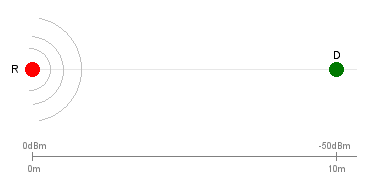
\includegraphics[width=\linewidth]{ideal.png}
\caption{Escenario ideal}
\label{fig:ideal}
\end{figure}

La imagen \ref{fig:ideal} presenta un escenario ideal en donde se tiene linea de visión entre el router transmisor \emph{R} y el dispositivo receptor \emph{D}, ubicados a una distancia de 10m uno del otro. La señal percibida en este ejemplo es de -25dBm.\\

\begin{figure}[h]
\centering
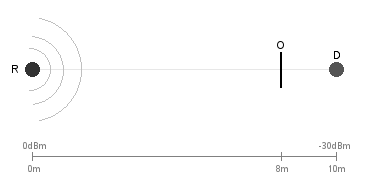
\includegraphics[width=\linewidth]{obstacle.png}
\caption{Escenario real}
\label{fig:obstacle}
\end{figure}

La imagen \ref{fig:obstacle} presenta un escenario un poco más realista, en donde la linea de visión se ve obstruida por un obstáculo \emph{O} (e.g. una pared) entre ellos. En este caso las ondas se ven perturbadas y el dispositivo solo percibe una señal de -30dBm, es decir, se tiene una atenuación de 5dBm.\\

\begin{figure}[h]
\centering
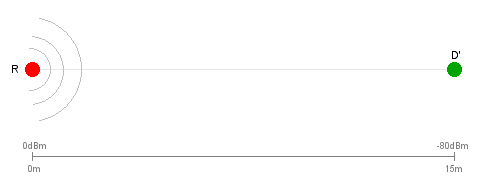
\includegraphics[width=\linewidth]{perceived.png}
\caption{Escenario percibido}
\label{fig:perceived}
\end{figure}

La imagen \ref{fig:perceived} representa la posición \emph{D'} en donde el dispositivo se percibiría a si mismo de no tener en cuenta posibles atenuaciones. Una señal de -30dBm será interpretada por él como una distancia de 12m en lugar de 10m, pero esto como no es real. El problema de fondo es la imposibilidad de determinar la existencia de obstáculos entre ambos extremos y como este afecta a la señal.\\

\subsubsection{Enfoque 1 - Atenuación Explícita}

Cada individuo es una n-úpla de la forma:

\begin{gather*}
I = (x, y, a_1, \dots, a_n)\\
x, y \in (-\infty, +\infty)\\
a_i \in [0, 1] \forall i \in (1, \dots, n)
\end{gather*}

En donde $(x,y)$ se corresponde con las coordenadas estimadas del individuo en el plano y los valores $a_i$ representan la atenuación estimada de la señal entre el dispositivo y el router \textit{i}.\\

De acuerdo a la representación descripta $(10, -5, 2.7, 0.0, 1.1)$ representa un individuo en una posición estimada $(10,-5)$ en el plano (con respecto al origen de coordenadas arbitrario usado para inicializar los routers) que tiene un decaimiento estimado de señal de 2.7dBm, 0.0dBm y 1.1dBm con respecto al router $R_1$, $R_2$ y $R_3$ respectivamente.\\

Si la intensidad de la señal que percibe de, por ejemplo, el router $R_1$ es de -30dBm, para el cálculo del fitness se asumiría que la misma debió ser 2.7dBm mayor, por lo cual se usará una señal teórica de $-30 + 2,7 = -27,3dBm$ en su lugar.\\

\begin{figure}[h]
\centering
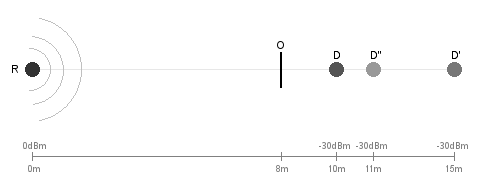
\includegraphics[width=\linewidth]{improvement.png}
\caption{Escenario mejorado}
\label{fig:improvement}
\end{figure}

La imagen \ref{fig:improvement} muestra el efecto que tiene sobre la estimación de la posición el hecho de considerar la atenuación hacia el router.\\

Al alterar la señal a partir de la atenuación estimada, el dispositivo \emph{D''} se acerca a la posición real \emph{D}.\\

Este enfoque, si bien en un primero momento parecía adecuado, tiene un defecto importante. La representación interna del individuo contiene un valor de atenuación hacia cada uno de los routers, por lo que dado cualquier valor para $(x,y)$, el algoritmo será capaz de modificar dichos valores de manera que el fitness sea bueno. En otras palabras, sin importar la estimación de la posición, existirá un vector de atenuación que haga que el individuo sea aceptable, potencialmente mejor que otro cuya posición estimada es más acertada. Asimismo, la representación interna dependería directamente de la cantidad de routers usados ya que para cada uno de ellos se deberá estimar un decaimiento, ocasionando que rápidamente el espacio de búsqueda crezca al punto de que no se explore lo suficiente en tiempos razonables.\\

\subsubsection{Enfoque 2 - Atenuación Implícita}

Cada individuo es un par de la forma:

\begin{gather*}
I = (x, y)\\
x, y \in (-\infty, +\infty)
\end{gather*}

En donde $(x,y)$ se corresponde con las coordenadas estimadas del individuo en el plano.\\

Este segundo enfoque extiende al anterior haciendo un mejor uso de la información obtenida del modelo de propagación de ondas. La idea a grandes rasgos consiste en inferir cuál es el decaimiento debido a los obstáculos, de manera que no sea necesario que el algoritmo lo estime.\\

Para esto es importante notar que dado cualquier punto en el plano, existen dos valores de intensidad de señal. Por un lado se tiene la \emph{señal teórica}, que corresponde a la señal que debería estar llegando en un escenario ideal y queda determinada únicamente a partir de la distancia entre el transmisor y el receptor. Por otro lado se tiene la \emph{señal recibida}, que corresponde a la \emph{señal teórica} menos un \emph{decaimiento} debido a obstáculos e interferencias.\\

De esta manera, la diferencia de ambas magnitudes es una buena aproximación del decaimiento usado en el enfoque anterior.

$$a_i = signal(\sqrt{(R_x-x)^2+(R_y-y)^2}) - S_r$$

Este enfoque no requiere una representación interna dependiente de la cantidad de routers y solo se limita a ajustar la posición del dispositivo, logrando un espacio de búsqueda mucho más acotado, aunque infinito.\\

La idea de aquí en más será adoptar esta alternativa y minimizar el vector de decaimientos inferido, o equivalentemente, minimizar la suma de la diferencia entre la distancia estimada (calculada a partir de la posición $(x,y)$) y la distancia teórica (calculada a partir de la señal percibida) respecto a cada router.\\

Es importante recordar que esto se estará haciendo para más de un router al mismo tiempo, por lo que el algoritmo deberá encontrar un punto de equilibrio. Si bien el vector del óptimo global será mínimo, en principio no será nulo.\\

\subsection{Función de Fitness}

La función de fitness a minimizar es la suma de errores respecto a la distancia estimada y la distancia teórica (calculada usando el modelo de propagación de ondas \emph{free space propagation model}).\\

\begin{equation*}
\begin{split}
f(x, y) = \sum_{i=1}^{n} |\sqrt{(R_{i_x}-x)^2 + (R_{i_y}-y)^2} - distance(R_{i_s})|
\end{split}
\end{equation*}

En donde $(R_{i_x},R_{i_y})$ y $R_{i_s}$ son la posición y la intensidad de señal recibida del router $i$ respectivamente, mientras que $(x,y)$ es la posición estimada del dispositivo que se está triangulando.\\

La función de fitness así expresada es una aproximación de la suma de los errores reales. Si bien se espera que su valor se aproxime a 0, difícilmente llegará a anularse completamente ya que cualquier atenuación debido a un obstáculo o interferencia implica en algún sentido pérdida de información, imposibilitando lograr triangular al dispositivo con una precisión arbitrariamente grande.

\subsection{Inicialización}

Como se ha dicho antes, se asume que los routers comparten características similares, en particular, que el alcance máximo para todos ellos es de \textit{A} metros (en la práctica se encontró que dicho valor es aproximadamente 50m \cite{routers:range}).\\

La población será inicializada eligiendo valores aleatorios para $(x,y)$ de manera que todos los individuos comiencen dentro del cuadrado que circunscribe todos los círculos de centro $(R_{i_x}, R_{i_y})$ y radio \textit{A}.\\

De esta manera, durante la inicialización de la población los valores estarán limitados por:

\begin{alignat*}{2}
x_{min} = \min_{i=1} {R_{i_x} - A} &\quad x_{max} = \max_{i=1} {R_{i_x} + A} \\
y_{min} = \min_{i=1} {R_{i_y} - A} &\quad y_{max} = \max_{i=1} {R_{i_y} + A}
\end{alignat*}

\subsection{Operadores}

Dado que el espacio de búsqueda es bastante grande, resulta esencial mantener la diversidad hasta haber muestreado una amplia área del plano, ya que en principio se puede asumir la existencia de muchos óptimos locales. Dicho esto, los operadores que serán utilizados se describen a continuación.\\

\subsubsection{Selección}

Se usará selección por torneo, habiendo probado también selección por ranking y rouletta, obteniendo en todos los casos resultados similares.\\

\subsubsection{Cruzamiento}

El operador de cruzamiento promediará los valores de ambos padres.

$$x_3 = \frac {x_1 + x_2} {2} \quad y_3 = \frac {y_1 + y_2} {2}$$

\subsubsection{Mutación}

El operador de mutación alterará la posición de acuerdo a un valor aleatorio elegido en un determinado rango.

\begin{gather*}
x = x + k_1 \quad y = y + k_2\\
k_1, k_2 \in (n,m)
\end{gather*}

\subsubsection{Búsqueda Local}

Las distancias con las que se trabajan son del orden de unos pocos metros a algunas decenas de metros. Dadas estas magnitudes, un error de entre 5cm y 25cm son igual de aceptables. Por lo tanto no existe la necesidad de optimizar el individuo para alcanzar la mejor estimación posible en su entorno.\\

Se considerará que un individuo con errores de estos ordenes es suficientemente bueno, de modo que no será necesario intentar disminuir aún más dicho error.\\

\subsection{Reemplazo de Individuos}

Dadas las características del framework se decidió realizar el reemplazo poblacional luego de aplicado el operador de cruzamiento. Para esto se seleccionan los dos mejores individuos entre los padres y sus respectivos hijos, pudiendo ocurrir que el individuo descendiente reemplace a uno de sus padres si su fitness es mejor que el de ellos.\\

\subsection{Criterio de Parada}

A partir de lo dicho anteriormente parece razonable parar el algoritmo si se consigue un individuo cuya suma de errores (es decir, el valor de la función de fitness) es menor a 5cm.\\

Al mismo tiempo será necesario un límite en el número de generaciones con el objetivo de evitar que el algoritmo converja a un óptimo local en donde no puede lograr tal precisión, ocasionando que no termine de ejecutarse. Para evitar esto empíricamente se encontró que un límite de 100 generaciones es suficiente, ya que en la mayoría de las ejecuciones la generación del mejor individuo estaba por debajo de este límite.\\

\subsection{Mecanismo de Reparación}

Cabe señalar que los individuos son válidos desde el momento de su inicialización y los operadores aplicados no los corrompen, por lo que no hace falta un mecanismo de reparación o de descarte de individuos inválidos.

\section{Análisis Experimental}

\subsection{Instancias de Prueba}

Las instancias de prueba son generadas de manera de simular entornos realistas.\\

Para esto se define la posición real del dispositivo y cierta cantidad de routers en un círculo de centro $(0,0)$ y radio 15m.\\

Una vez hecho se tiene la posición de todos los nodos presentes se calcula la distancia real entre el dispositivo y cada uno de los routers. Mediante esta distancia y el modelo de propagación de ondas se obtiene la señal real que percibiría, a la cual se le substrae un valor aleatorio, correspondiente al decaimiento, de entre 0dBm y 2dBm.\\

\subsection{Entorno de Prueba}

Dado que en la práctica la implementación realizada no parece necesitar de grandes tiempos de ejecución ni grandes cantidades de memoria o procesamiento que requieran correrlo en un cluster, se usará una computadora de características moderadas para realizar las pruebas.\\

\subsubsection{Marca y Modelo}

Dell Inspiron N5010\\

\subsubsection{Procesador}

Intel Core i5 2.67GHz (doble nucleo, cuatro threads), 64KB de cache L1, 512KB de cache L2, 3MB de cache L3\\

\subsubsection{Memoria}

4GB de memoria DDR3 1333MHz\\

\subsubsection{Sistema Operativo}

\emph{GNU/Linux} \cite{gnu} \cite{linux}, en su variante \emph{Debian 7.0 Wheezy} \cite{debian:stable} para 64 bits (amd64).\\

Se prestó especial cuidado a los procesos ejecutándose, deteniendo todos las aplicaciones y servicios innecesarios al momento de realizar las pruebas.

\subsection{Ajuste Paramétrico}

Para el ajuste paramétrico se usará una instancia de prueba reducida, conformada por 3 routers ubicados aleatoriamente en el plano. A partir de dicha instancia y para cada combinación de parámetros se harán 3 ejecuciones independientes.\\

La tabla \ref{tab:tuning} muestra las combinaciones de parámetros estudiados para hacer el ajuste paramétrico, el fitness corresponde al mejor individuo encontrado en las 5 ejecuciones independientes.

\begin{table}[h]
\caption{Ajuste paramétrico}
\centering
\begin{tabular}{|c|c|c||r|}
\hline
Población &Cruzamiento &Mutación &Fitness \\
\hline
\multirow{9}{*}{5}  & \multirow{3}{*}{0.70} & 0.01 & 0.4776 \\
                    &                       & 0.05 & 0.2555 \\
                    &                       & 0.10 & 0.3230 \\ \cline{2-4}
                    & \multirow{3}{*}{0.80} & 0.01 & 0.3166 \\
                    &                       & 0.05 & 0.3383 \\
                    &                       & 0.10 & 0.2588 \\ \cline{2-4}
                    & \multirow{3}{*}{0.90} & 0.01 & 0.2606 \\
                    &                       & 0.05 & 0.2965 \\
                    &                       & 0.10 & 0.2566 \\ \hline
\multirow{9}{*}{15} & \multirow{3}{*}{0.70} & 0.01 & 0.2707 \\
                    &                       & 0.05 & 0.3181 \\
                    &                       & 0.10 & 0.2558 \\ \cline{2-4}
                    & \multirow{3}{*}{0.80} & 0.01 & 0.2623 \\
                    &                       & 0.05 & 0.2568 \\
                    &                       & 0.10 & 0.2561 \\ \cline{2-4}
                    & \multirow{3}{*}{0.90} & 0.01 & 0.2701 \\
                    &                       & 0.05 & 0.2605 \\
                    &                       & 0.10 & 0.2553 \\ \hline
\multirow{9}{*}{30} & \multirow{3}{*}{0.70} & 0.01 & 0.2559 \\
                    &                       & 0.05 & 0.2554 \\
                    &                       & 0.10 & 0.2553 \\ \cline{2-4}
                    & \multirow{3}{*}{0.80} & 0.01 & 0.3199 \\
                    &                       & 0.05 & 0.2554 \\
                    &                       & 0.10 & 0.2554 \\ \cline{2-4}
                    & \multirow{3}{*}{0.90} & 0.01 & 0.3194 \\
                    &                       & 0.05 & 0.2561 \\
                    &                       & 0.10 & 0.2554 \\ \hline
\end{tabular}
\label{tab:tuning}
\end{table}

\begin{figure}[h]
\centering
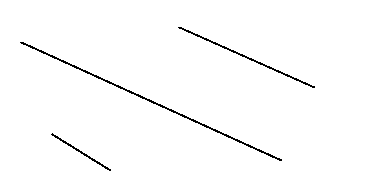
\includegraphics[width=\linewidth]{fitness_generations.png}
\caption{Evolución del fitness en función de la generación}
\label{fig:fitness_generations}
\end{figure}

\subsubsection*{Análisis}

A partir de los resultados obtenidos se puede apreciar como, para todas las combinaciones de parámetros con los que se probó, las soluciones son muy buenas. Existe cierta tendencia a obtener soluciones marginalmente peores para una probabilidad de cruzamiento 0.01, en especial combinando esto con poblaciones chicas, una posible explicación de este fenómeno es la diversidad.\\

Con el objetivo de obtener soluciones de calidad y al mismo tiempo mantener la diversidad en la población se optará de aquí en más por una población de 30 individuos, una probabilidad de 0.9 para el operador de cruzamiento y de 0.1 para el operador de mutación.\\

\subsubsection*{Análisis de Normalidad}

\begin{figure}[h]
\centering
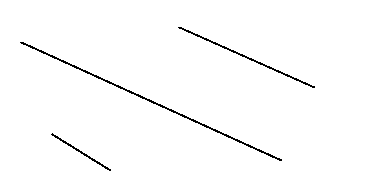
\includegraphics[width=\linewidth]{distribution.png}
\caption{Distribución de la probabilidad de fitness}
\label{fig:distribution}
\end{figure}

El análisis de normalidad dió negativo.

\subsection{Evaluación}

Para realizar la evaluación del algoritmo se usarán 25 instancias de prueba divididas en 5 conjuntos de 3, 4, 5, 6 y 7 routers. Para cada instancia se harán 5 ejecuciones independientes, completando en total 125 ejecuciones.\\

Para todos los casos se reportará:\\

\begin{itemize}
\item $G$: generación del mejor individuo ($I$)
\item $f$: fitness de $I$
\item $f_{AVG}$: promedio de fitness de los individuos de $G$
\item $\sigma_f$: desviación estándar de los individuos de $G$
\item $t$: segundos utilizados para encontrar $I$
\item $t_{AVG}$: promedio de $t$ para todas las ejecuciones
\item $\sigma_t$: desviación estándar de $t$ para todas las ejecuciones
\item $Error$: error en metros respecto de la posición real
\end{itemize}

\begin{table}[h]
\caption{Resultados}
\centering

\begin{tabular}{|c||c||c|c|c||c|c|c||c|}
\hline
$R$ & $G$ & $f$ & $f_{AVG}$ & $\sigma_f$ & $t$ & $t_{AVG}$ & $\sigma_t$ & $Error$ \\
\hline
\multirow{5}{*}{3} & 63 & 0.8010 & 0.8143 & 0.0432 & 0.0025 & 0.0029 & 0.0012 & 2.3242 \\
                   & 32 & 0.0673 & 0.0673 & 0.0000 & 0.0013 & 0.0027 & 0.0010 & 0.4029 \\
                   & 37 & 0.1235 & 0.1344 & 0.0588 & 0.0015 & 0.0032 & 0.0009 & 0,4697 \\
                   & 67 & 0.2488 & 0.2675 & 0.0346 & 0.0026 & 0.0027 & 0.0011 & 1.8703 \\
                   & 93 & 0.9314 & 0.9398 & 0.0260 & 0.0037 & 0.0028 & 0.0009 & 0.2762 \\ \hline

\multirow{5}{*}{4} & 68 & 0.5443 & 0.5635 & 0.0926 & 0.0033 & 0.0038 & 0.0012 & 3.7109 \\
                   & 64 & 4.6128 & 4.6148 & 0.0035 & 0.0032 & 0.0039 & 0.0011 & 0.9137 \\
                   & 66 & 0.9033 & 0.9909 & 0.3262 & 0.0033 & 0.0040 & 0.0012 & 1.7610 \\
                   & 72 & 0.4688 & 0.5045 & 0.1170 & 0.0036 & 0.0039 & 0.0011 & 1.0826 \\
                   & 73 & 0.5379 & 0.5379 & 0.0000 & 0.0037 & 0.0034 & 0.0013 & 1.2822 \\ \hline
 
\multirow{5}{*}{5} & 84 & 1.5151 & 1.6268 & 0.3751 & 0.0050 & 0.0050 & 0.0014 & 1.9611 \\
                   & 75 & 3.2720 & 3.5045 & 0.3604 & 0.0046 & 0.0053 & 0.0019 & 1.5947 \\
                   & 97 & 1.9190 & 2.2812 & 1.0508 & 0.0058 & 0.0044 & 0.0014 & 1.1976 \\
                   & 91 & 2.0561 & 2.0658 & 0.0367 & 0.0054 & 0.0048 & 0.0011 & 1.7748 \\
                   & 78 & 1.3183 & 1.3658 & 0.1710 & 0.0046 & 0.0044 & 0.0013 & 2.9317 \\ \hline
 
\multirow{5}{*}{6} & 91 & 1.9640 & 2.1919 & 0.5130 & 0.0064 & 0.0052 & 0.0015 & 0.2240 \\
                   & 80 & 2.0648 & 2.0938 & 0.0719 & 0.0056 & 0.0052 & 0.0013 & 1.4460 \\
                   & 56 & 3.9024 & 3.9758 & 0.4020 & 0.0040 & 0.0056 & 0.0012 & 1.6684 \\
                   & 74 & 4.0438 & 4.1785 & 0.3956 & 0.0052 & 0.0051 & 0.0016 & 1.3792 \\
                   & 63 & 0.3889 & 0.4289 & 0.2195 & 0.0045 & 0.0053 & 0.0024 & 2.4719 \\ \hline
 
\multirow{5}{*}{7} & 46 & 1.6373 & 1.6449 & 0.0139 & 0.0037 & 0.0060 & 0.0018 & 0.9565 \\
                   & 66 & 1.0254 & 1.0827 & 0.1501 & 0.0053 & 0.0061 & 0.0017 & 0.8127 \\
                   & 63 & 1.8974 & 1.8975 & 0.0000 & 0.0051 & 0.0062 & 0.0016 & 1.2088 \\
                   & 95 & 3.3067 & 3.3073 & 0.0034 & 0.0076 & 0.0061 & 0.0017 & 1.5144 \\
                   & 58 & 5.4602 & 5.4837 & 0.0833 & 0.0047 & 0.0059 & 0.0020 & 1.3776 \\  \hline

\end{tabular}

\label{tab:evaluation}
\end{table}

\begin{figure}[h]
\centering
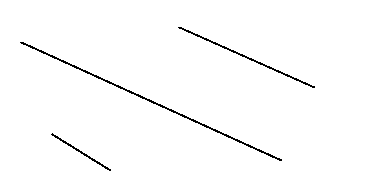
\includegraphics[width=\linewidth]{generations.png}
\caption{Generación de los mejores individuos}
\label{fig:generations}
\end{figure}

\begin{figure}[h]
\centering
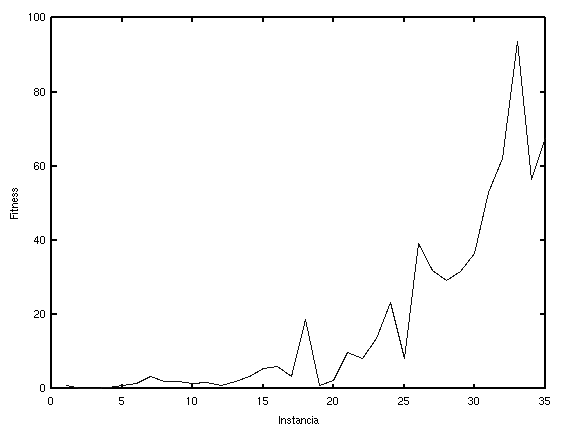
\includegraphics[width=\linewidth]{fitness.png}
\caption{Fitness de los mejores individuos}
\label{fig:fitness}
\end{figure}

\begin{figure}[h]
\centering
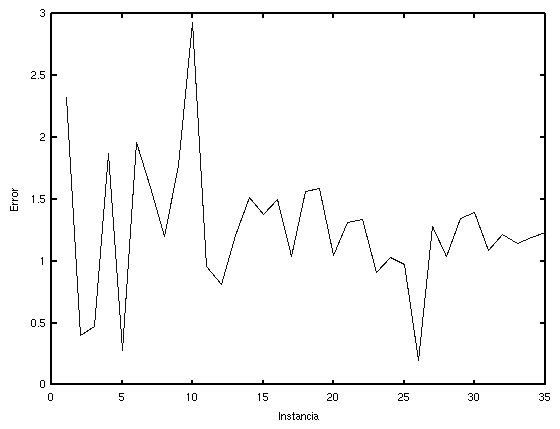
\includegraphics[width=\linewidth]{errors.png}
\caption{Errores reales de los mejores individuos}
\label{fig:errors}
\end{figure}

\subsubsection*{Análisis}

Todas las soluciones obtenidas son muy buenas, presentando en general errores del orden de 1m. Por otro lado los tiempos de ejecución son muy cortos, evidenciando la capacidad del algoritmo implementado para hallar rápidamente una excelente aproximación de la posición real del dispositivo.\\

A partir del fitness de los mejores individuos y de las generaciones en las que fueron encontrados parece correcto afirmar que aunque se corriera el algoritmo por más tiempo no sería posible mejorar el error. De hecho, parece estar encontrando las mejores soluciones posibles, pero está sujeto a la falta de información debido a las atenuaciones existentes.\\

A medida que aumenta la cantidad de routers se mejora marginalmente los resultados, aún así cabe señalar la variación de errores para instancias de prueba con la misma cantidad de routers, lo cual es razonable ya que una correcta triangulación depende en gran medida de la posición relativa de los nodos.\\

En general, parece primar la imprecisión intrínseca del modelo elegido, no pudiendo mejorar arbitrariamente la precisión, como se había predecido en un principio.\\

\section{Conclusión}

A juzgar por los resultados obtenidos en el análisis experimental se puede concluir la validez de la propuesta de usar algoritmos evolutivos para triangular nodos inalámbricos.\\

Como se evidencia para cada uno de los casos de prueba usados, el algoritmo fue capaz de encontrar una aproximación bastante precisa de la posición real del dispositivo. Si bien esta aproximación está limitada por incertidumbres en las mediciones y sesgada por el modelo de propagación de ondas usado, se demostró la posibilidad de triangular dispositivos móviles en tiempos muy reducidos.\\

Concluimos que un enfoque como el presentado aquí perfectamente puede ser usado en la práctica si se cuenta con al menos tres routers de los cuales sí se conoce su ubicación.\\

\section{Trabajo Futuro}

Durante el análisis del problema se hicieron varias suposiciones, que si bien son adecuadas en el contexto en el que se trabaja, no dejan de ser una simplificación de la realidad.\\

En el futuro se debería adoptar otro modelo de propagación de ondas más sofisticado con el objetivo de ver de que manera esto influye en las soluciones encontradas por el algoritmo.\\

Además de esto sería interesante triangular a los dispositivos en un espacio tridimencional, lo que requeriría agregar una nueva coordenada a la representación interna de los individuos y tener ciertas consideraciones especiales respecto a las antenas.\\

Por último, por no contar con el equipo adecuado y los medios para realizar mediciones suficientemente precisas se optó por limitarse a la simulación de triangulaciones con ejemplos generados aleatoriamente. En un futuro se deberá poner a prueba la propuesta utilizando routers reales en un ambiente controlado, con el objetivo de poner a prueba la validez del estudio realizado.\\

\newpage

% trigger a \newpage just before the given reference
% number - used to balance the columns on the last page
% adjust value as needed - may need to be readjusted if
% the document is modified later
%\IEEEtriggeratref{8}
% The "triggered" command can be changed if desired:
%\IEEEtriggercmd{\enlargethispage{-5in}}

% references section

% can use a bibliography generated by BibTeX as a .bbl file
% BibTeX documentation can be easily obtained at:
% http://www.ctan.org/tex-archive/biblio/bibtex/contrib/doc/
% The IEEEtran BibTeX style support page is at:
% http://www.michaelshell.org/tex/ieeetran/bibtex/
%\bibliographystyle{IEEEtran}
% argument is your BibTeX string definitions and bibliography database(s)
%\bibliography{IEEEabrv,../bib/paper}
%
% <OR> manually copy in the resultant .bbl file
% set second argument of \begin to the number of references
% (used to reserve space for the reference number labels box)

\bibliographystyle{unsrt}
\bibliography{refs}

% You can push biographies down or up by placing
% a \vfill before or after them. The appropriate
% use of \vfill depends on what kind of text is
% on the last page and whether or not the columns
% are being equalized.

%\vfill

% Can be used to pull up biographies so that the bottom of the last one
% is flush with the other column.
%\enlargethispage{-5in}



% that's all folks
\end{document}